\documentclass[1p]{elsarticle_modified}
%\bibliographystyle{elsarticle-num}

%\usepackage[colorlinks]{hyperref}
%\usepackage{abbrmath_seonhwa} %\Abb, \Ascr, \Acal ,\Abf, \Afrak
\usepackage{amsfonts}
\usepackage{amssymb}
\usepackage{amsmath}
\usepackage{amsthm}
\usepackage{scalefnt}
\usepackage{amsbsy}
\usepackage{kotex}
\usepackage{caption}
\usepackage{subfig}
\usepackage{color}
\usepackage{graphicx}
\usepackage{xcolor} %% white, black, red, green, blue, cyan, magenta, yellow
\usepackage{float}
\usepackage{setspace}
\usepackage{hyperref}

\usepackage{tikz}
\usetikzlibrary{arrows}

\usepackage{multirow}
\usepackage{array} % fixed length table
\usepackage{hhline}

%%%%%%%%%%%%%%%%%%%%%
\makeatletter
\renewcommand*\env@matrix[1][\arraystretch]{%
	\edef\arraystretch{#1}%
	\hskip -\arraycolsep
	\let\@ifnextchar\new@ifnextchar
	\array{*\c@MaxMatrixCols c}}
\makeatother %https://tex.stackexchange.com/questions/14071/how-can-i-increase-the-line-spacing-in-a-matrix
%%%%%%%%%%%%%%%

\usepackage[normalem]{ulem}

\newcommand{\msout}[1]{\ifmmode\text{\sout{\ensuremath{#1}}}\else\sout{#1}\fi}
%SOURCE: \msout is \stkout macro in https://tex.stackexchange.com/questions/20609/strikeout-in-math-mode

\newcommand{\cancel}[1]{
	\ifmmode
	{\color{red}\msout{#1}}
	\else
	{\color{red}\sout{#1}}
	\fi
}

\newcommand{\add}[1]{
	{\color{blue}\uwave{#1}}
}

\newcommand{\replace}[2]{
	\ifmmode
	{\color{red}\msout{#1}}{\color{blue}\uwave{#2}}
	\else
	{\color{red}\sout{#1}}{\color{blue}\uwave{#2}}
	\fi
}

\newcommand{\Sol}{\mathcal{S}} %segment
\newcommand{\D}{D} %diagram
\newcommand{\A}{\mathcal{A}} %arc


%%%%%%%%%%%%%%%%%%%%%%%%%%%%%5 test

\def\sl{\operatorname{\textup{SL}}(2,\Cbb)}
\def\psl{\operatorname{\textup{PSL}}(2,\Cbb)}
\def\quan{\mkern 1mu \triangleright \mkern 1mu}

\theoremstyle{definition}
\newtheorem{thm}{Theorem}[section]
\newtheorem{prop}[thm]{Proposition}
\newtheorem{lem}[thm]{Lemma}
\newtheorem{ques}[thm]{Question}
\newtheorem{cor}[thm]{Corollary}
\newtheorem{defn}[thm]{Definition}
\newtheorem{exam}[thm]{Example}
\newtheorem{rmk}[thm]{Remark}
\newtheorem{alg}[thm]{Algorithm}

\newcommand{\I}{\sqrt{-1}}
\begin{document}

%\begin{frontmatter}
%
%\title{Boundary parabolic representations of knots up to 8 crossings}
%
%%% Group authors per affiliation:
%\author{Yunhi Cho} 
%\address{Department of Mathematics, University of Seoul, Seoul, Korea}
%\ead{yhcho@uos.ac.kr}
%
%
%\author{Seonhwa Kim} %\fnref{s_kim}}
%\address{Center for Geometry and Physics, Institute for Basic Science, Pohang, 37673, Korea}
%\ead{ryeona17@ibs.re.kr}
%
%\author{Hyuk Kim}
%\address{Department of Mathematical Sciences, Seoul National University, Seoul 08826, Korea}
%\ead{hyukkim@snu.ac.kr}
%
%\author{Seokbeom Yoon}
%\address{Department of Mathematical Sciences, Seoul National University, Seoul, 08826,  Korea}
%\ead{sbyoon15@snu.ac.kr}
%
%\begin{abstract}
%We find all boundary parabolic representation of knots up to 8 crossings.
%
%\end{abstract}
%\begin{keyword}
%    \MSC[2010] 57M25 
%\end{keyword}
%
%\end{frontmatter}

%\linenumbers
%\tableofcontents
%
\newcommand\colored[1]{\textcolor{white}{\rule[-0.35ex]{0.8em}{1.4ex}}\kern-0.8em\color{red} #1}%
%\newcommand\colored[1]{\textcolor{white}{ #1}\kern-2.17ex	\textcolor{white}{ #1}\kern-1.81ex	\textcolor{white}{ #1}\kern-2.15ex\color{red}#1	}

{\Large $\underline{12n_{0491}~(K12n_{0491})}$}

\setlength{\tabcolsep}{10pt}
\renewcommand{\arraystretch}{1.6}
\vspace{1cm}\begin{tabular}{m{100pt}>{\centering\arraybackslash}m{274pt}}
\multirow{5}{120pt}{
	\centering
	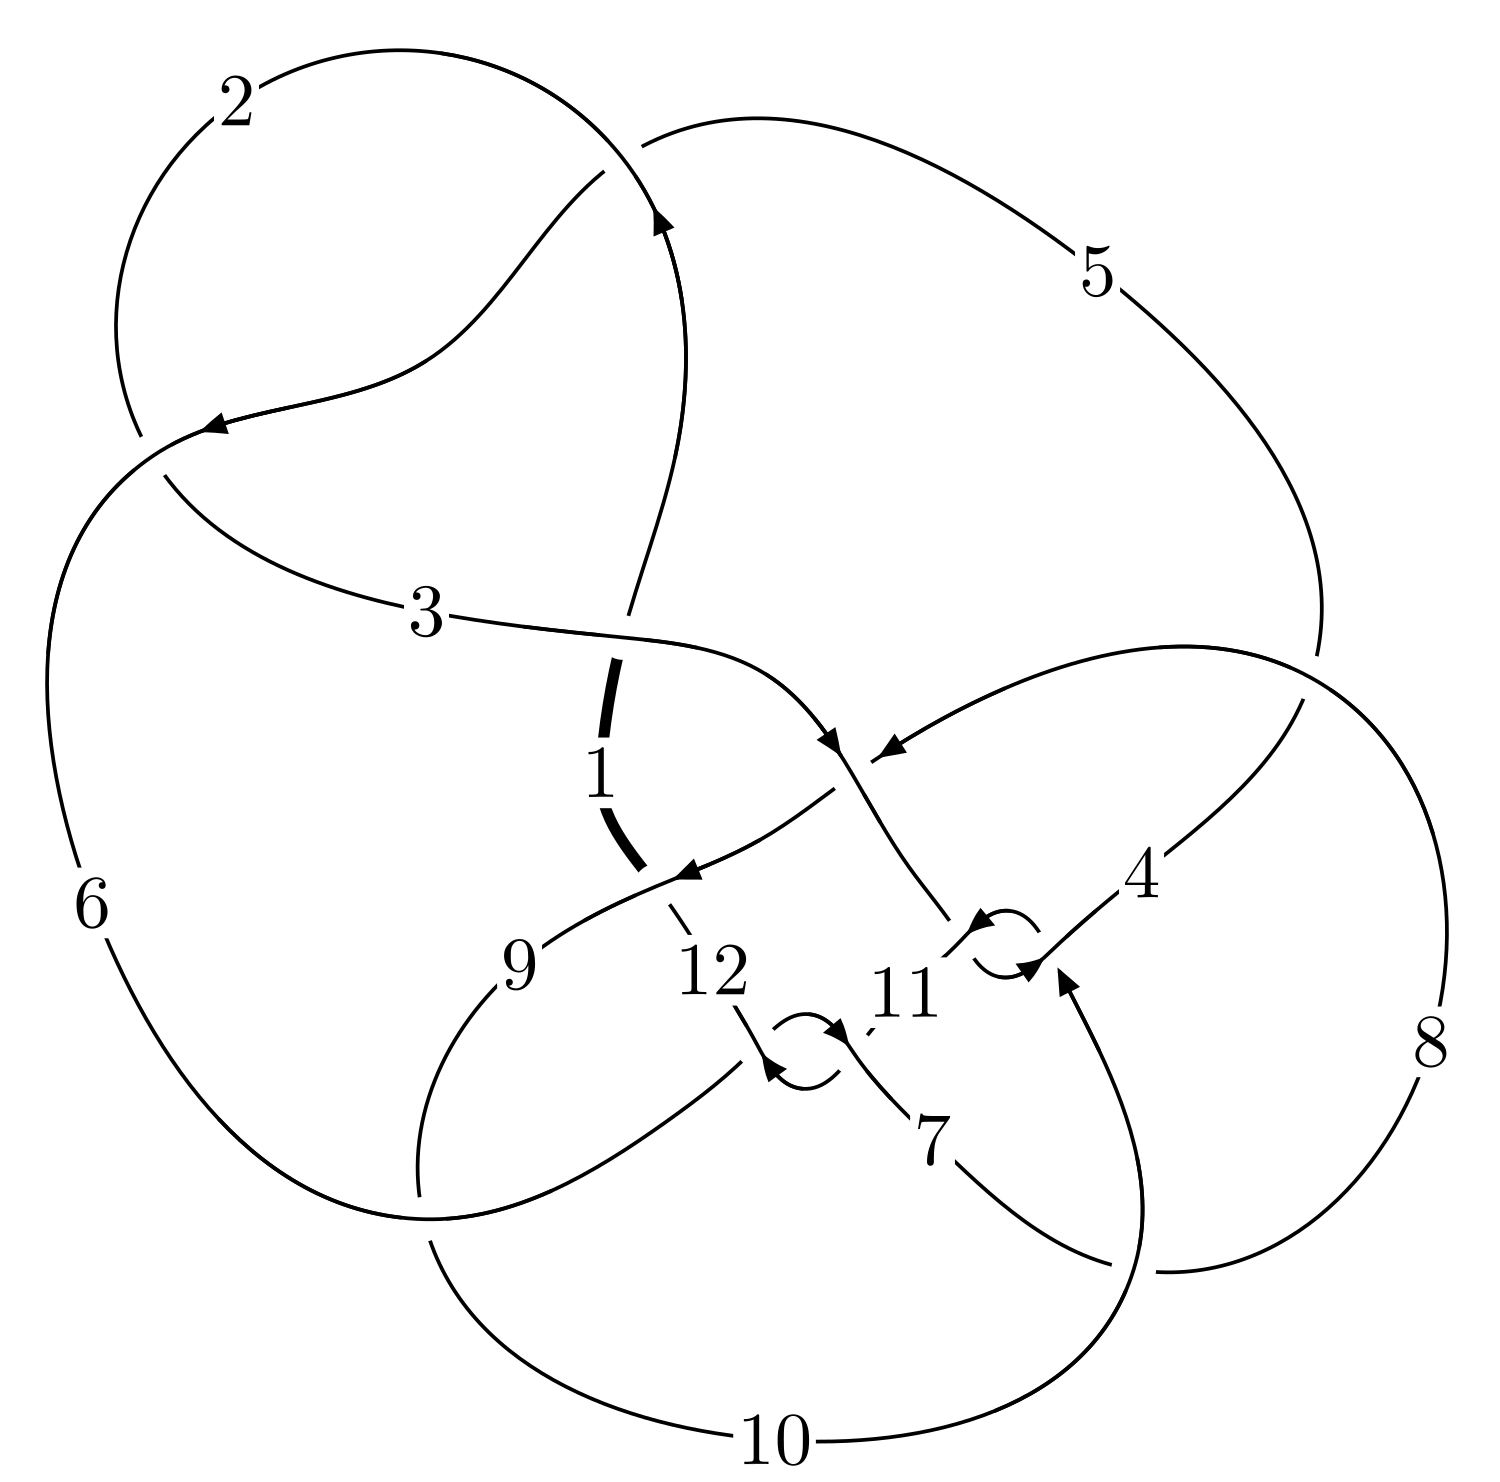
\includegraphics[width=112pt]{../../../GIT/diagram.site/Diagrams/png/2580_12n_0491.png}\\
\ \ \ A knot diagram\footnotemark}&
\allowdisplaybreaks
\textbf{Linearized knot diagam} \\
\cline{2-2}
 &
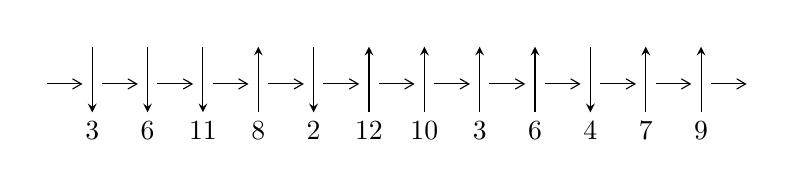
\begin{tikzpicture}[x=20pt, y=17pt]
	% nodes
	\node (C0) at (0, 0) {};
	\node (C1) at (1, 0) {};
	\node (C1U) at (1, +1) {};
	\node (C1D) at (1, -1) {3};

	\node (C2) at (2, 0) {};
	\node (C2U) at (2, +1) {};
	\node (C2D) at (2, -1) {6};

	\node (C3) at (3, 0) {};
	\node (C3U) at (3, +1) {};
	\node (C3D) at (3, -1) {11};

	\node (C4) at (4, 0) {};
	\node (C4U) at (4, +1) {};
	\node (C4D) at (4, -1) {8};

	\node (C5) at (5, 0) {};
	\node (C5U) at (5, +1) {};
	\node (C5D) at (5, -1) {2};

	\node (C6) at (6, 0) {};
	\node (C6U) at (6, +1) {};
	\node (C6D) at (6, -1) {12};

	\node (C7) at (7, 0) {};
	\node (C7U) at (7, +1) {};
	\node (C7D) at (7, -1) {10};

	\node (C8) at (8, 0) {};
	\node (C8U) at (8, +1) {};
	\node (C8D) at (8, -1) {3};

	\node (C9) at (9, 0) {};
	\node (C9U) at (9, +1) {};
	\node (C9D) at (9, -1) {6};

	\node (C10) at (10, 0) {};
	\node (C10U) at (10, +1) {};
	\node (C10D) at (10, -1) {4};

	\node (C11) at (11, 0) {};
	\node (C11U) at (11, +1) {};
	\node (C11D) at (11, -1) {7};

	\node (C12) at (12, 0) {};
	\node (C12U) at (12, +1) {};
	\node (C12D) at (12, -1) {9};
	\node (C13) at (13, 0) {};

	% arrows
	\draw[->,>={angle 60}]
	(C0) edge (C1) (C1) edge (C2) (C2) edge (C3) (C3) edge (C4) (C4) edge (C5) (C5) edge (C6) (C6) edge (C7) (C7) edge (C8) (C8) edge (C9) (C9) edge (C10) (C10) edge (C11) (C11) edge (C12) (C12) edge (C13) ;	\draw[->,>=stealth]
	(C1U) edge (C1D) (C2U) edge (C2D) (C3U) edge (C3D) (C4D) edge (C4U) (C5U) edge (C5D) (C6D) edge (C6U) (C7D) edge (C7U) (C8D) edge (C8U) (C9D) edge (C9U) (C10U) edge (C10D) (C11D) edge (C11U) (C12D) edge (C12U) ;
	\end{tikzpicture} \\
\hhline{~~} \\& 
\textbf{Solving Sequence} \\ \cline{2-2} 
 &
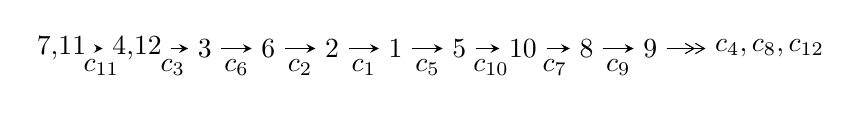
\begin{tikzpicture}[x=23pt, y=7pt]
	% node
	\node (A0) at (-1/8, 0) {7,11};
	\node (A1) at (17/16, 0) {4,12};
	\node (A2) at (17/8, 0) {3};
	\node (A3) at (25/8, 0) {6};
	\node (A4) at (33/8, 0) {2};
	\node (A5) at (41/8, 0) {1};
	\node (A6) at (49/8, 0) {5};
	\node (A7) at (57/8, 0) {10};
	\node (A8) at (65/8, 0) {8};
	\node (A9) at (73/8, 0) {9};
	\node (C1) at (1/2, -1) {$c_{11}$};
	\node (C2) at (13/8, -1) {$c_{3}$};
	\node (C3) at (21/8, -1) {$c_{6}$};
	\node (C4) at (29/8, -1) {$c_{2}$};
	\node (C5) at (37/8, -1) {$c_{1}$};
	\node (C6) at (45/8, -1) {$c_{5}$};
	\node (C7) at (53/8, -1) {$c_{10}$};
	\node (C8) at (61/8, -1) {$c_{7}$};
	\node (C9) at (69/8, -1) {$c_{9}$};
	\node (A10) at (11, 0) {$c_{4},c_{8},c_{12}$};

	% edge
	\draw[->,>=stealth]	
	(A0) edge (A1) (A1) edge (A2) (A2) edge (A3) (A3) edge (A4) (A4) edge (A5) (A5) edge (A6) (A6) edge (A7) (A7) edge (A8) (A8) edge (A9) ;
	\draw[->>,>={angle 60}]	
	(A9) edge (A10);
\end{tikzpicture} \\ 

\end{tabular} \\

\footnotetext{
The image of knot diagram is generated by the software ``\textbf{Draw programme}" developed by Andrew Bartholomew(\url{http://www.layer8.co.uk/maths/draw/index.htm\#Running-draw}), where we modified some parts for our purpose(\url{https://github.com/CATsTAILs/LinksPainter}).
}\phantom \\ \newline 
\centering \textbf{Ideals for irreducible components\footnotemark of $X_{\text{par}}$} 
 
\begin{align*}
I^u_{1}&=\langle 
-6.28259\times10^{69} u^{52}-3.92104\times10^{70} u^{51}+\cdots+1.58927\times10^{71} b+7.23259\times10^{71},\\
\phantom{I^u_{1}}&\phantom{= \langle  }-1.12367\times10^{72} u^{52}+1.44284\times10^{72} u^{51}+\cdots+3.01961\times10^{72} a+1.87033\times10^{73},\\
\phantom{I^u_{1}}&\phantom{= \langle  }u^{53}-2 u^{52}+\cdots-40 u-19\rangle \\
I^u_{2}&=\langle 
-13796 u^{18}-18331 u^{17}+\cdots+45431 b+86665,\\
\phantom{I^u_{2}}&\phantom{= \langle  }172722 u^{18}+249659 u^{17}+\cdots+318017 a-540027,\;u^{19}+u^{18}+\cdots-3 u-7\rangle \\
\\
\end{align*}
\raggedright * 2 irreducible components of $\dim_{\mathbb{C}}=0$, with total 72 representations.\\
\footnotetext{All coefficients of polynomials are rational numbers. But the coefficients are sometimes approximated in decimal forms when there is not enough margin.}
\newpage
\renewcommand{\arraystretch}{1}
\centering \section*{I. $I^u_{1}= \langle -6.28\times10^{69} u^{52}-3.92\times10^{70} u^{51}+\cdots+1.59\times10^{71} b+7.23\times10^{71},\;-1.12\times10^{72} u^{52}+1.44\times10^{72} u^{51}+\cdots+3.02\times10^{72} a+1.87\times10^{73},\;u^{53}-2 u^{52}+\cdots-40 u-19 \rangle$}
\flushleft \textbf{(i) Arc colorings}\\
\begin{tabular}{m{7pt} m{180pt} m{7pt} m{180pt} }
\flushright $a_{7}=$&$\begin{pmatrix}0\\u\end{pmatrix}$ \\
\flushright $a_{11}=$&$\begin{pmatrix}1\\0\end{pmatrix}$ \\
\flushright $a_{4}=$&$\begin{pmatrix}0.372124 u^{52}-0.477822 u^{51}+\cdots-20.2423 u-6.19396\\0.0395313 u^{52}+0.246720 u^{51}+\cdots-9.19809 u-4.55090\end{pmatrix}$ \\
\flushright $a_{12}=$&$\begin{pmatrix}1\\- u^2\end{pmatrix}$ \\
\flushright $a_{3}=$&$\begin{pmatrix}0.411656 u^{52}-0.231102 u^{51}+\cdots-29.4404 u-10.7449\\0.0395313 u^{52}+0.246720 u^{51}+\cdots-9.19809 u-4.55090\end{pmatrix}$ \\
\flushright $a_{6}=$&$\begin{pmatrix}- u\\u^3+u\end{pmatrix}$ \\
\flushright $a_{2}=$&$\begin{pmatrix}0.458907 u^{52}-0.728958 u^{51}+\cdots-18.2819 u-5.32838\\0.0479872 u^{52}+0.108330 u^{51}+\cdots-5.12020 u-2.30366\end{pmatrix}$ \\
\flushright $a_{1}=$&$\begin{pmatrix}-0.217784 u^{52}-1.10568 u^{51}+\cdots+53.3268 u+23.0233\\-0.0127121 u^{52}-1.28483 u^{51}+\cdots+42.1962 u+19.5101\end{pmatrix}$ \\
\flushright $a_{5}=$&$\begin{pmatrix}-0.486443 u^{52}+0.781036 u^{51}+\cdots+16.1784 u+4.41592\\0.210529 u^{52}-0.0287556 u^{51}+\cdots-14.2682 u-5.35874\end{pmatrix}$ \\
\flushright $a_{10}=$&$\begin{pmatrix}-0.151735 u^{52}+0.441502 u^{51}+\cdots-4.60673 u-1.92073\\0.621884 u^{52}-1.11241 u^{51}+\cdots-9.54706 u-0.104321\end{pmatrix}$ \\
\flushright $a_{8}=$&$\begin{pmatrix}0.124913 u^{52}-0.625193 u^{51}+\cdots+8.69636 u+6.25801\\-0.0892206 u^{52}+0.468833 u^{51}+\cdots-9.12061 u-4.72212\end{pmatrix}$ \\
\flushright $a_{9}=$&$\begin{pmatrix}0.642220 u^{52}-0.865075 u^{51}+\cdots-19.8419 u-3.61549\\0.832643 u^{52}-1.27823 u^{51}+\cdots-20.6504 u-3.75489\end{pmatrix}$\\&\end{tabular}
\flushleft \textbf{(ii) Obstruction class $= -1$}\\~\\
\flushleft \textbf{(iii) Cusp Shapes $= 0.0970191 u^{52}+0.877677 u^{51}+\cdots-34.0551 u-20.3470$}\\~\\
\newpage\renewcommand{\arraystretch}{1}
\flushleft \textbf{(iv) u-Polynomials at the component}\newline \\
\begin{tabular}{m{50pt}|m{274pt}}
Crossings & \hspace{64pt}u-Polynomials at each crossing \\
\hline $$\begin{aligned}c_{1}\end{aligned}$$&$\begin{aligned}
&u^{53}+78 u^{52}+\cdots+5037 u+49
\end{aligned}$\\
\hline $$\begin{aligned}c_{2},c_{5}\end{aligned}$$&$\begin{aligned}
&u^{53}+6 u^{52}+\cdots+173 u-7
\end{aligned}$\\
\hline $$\begin{aligned}c_{3},c_{10}\end{aligned}$$&$\begin{aligned}
&u^{53}+2 u^{52}+\cdots-17 u-13
\end{aligned}$\\
\hline $$\begin{aligned}c_{4}\end{aligned}$$&$\begin{aligned}
&u^{53}-3 u^{52}+\cdots+34374 u-17789
\end{aligned}$\\
\hline $$\begin{aligned}c_{6},c_{11}\end{aligned}$$&$\begin{aligned}
&u^{53}-2 u^{52}+\cdots-40 u-19
\end{aligned}$\\
\hline $$\begin{aligned}c_{7}\end{aligned}$$&$\begin{aligned}
&u^{53}+16 u^{52}+\cdots-1526 u-127
\end{aligned}$\\
\hline $$\begin{aligned}c_{8}\end{aligned}$$&$\begin{aligned}
&u^{53}+u^{52}+\cdots+307064 u-83053
\end{aligned}$\\
\hline $$\begin{aligned}c_{9}\end{aligned}$$&$\begin{aligned}
&u^{53}-4 u^{52}+\cdots-9953511 u-5353931
\end{aligned}$\\
\hline $$\begin{aligned}c_{12}\end{aligned}$$&$\begin{aligned}
&u^{53}+44 u^{51}+\cdots-895504 u-204397
\end{aligned}$\\
\hline
\end{tabular}\\~\\
\newpage\renewcommand{\arraystretch}{1}
\flushleft \textbf{(v) Riley Polynomials at the component}\newline \\
\begin{tabular}{m{50pt}|m{274pt}}
Crossings & \hspace{64pt}Riley Polynomials at each crossing \\
\hline $$\begin{aligned}c_{1}\end{aligned}$$&$\begin{aligned}
&y^{53}-198 y^{52}+\cdots+8975185 y-2401
\end{aligned}$\\
\hline $$\begin{aligned}c_{2},c_{5}\end{aligned}$$&$\begin{aligned}
&y^{53}-78 y^{52}+\cdots+5037 y-49
\end{aligned}$\\
\hline $$\begin{aligned}c_{3},c_{10}\end{aligned}$$&$\begin{aligned}
&y^{53}+34 y^{52}+\cdots-23 y-169
\end{aligned}$\\
\hline $$\begin{aligned}c_{4}\end{aligned}$$&$\begin{aligned}
&y^{53}+27 y^{52}+\cdots-3258740414 y-316448521
\end{aligned}$\\
\hline $$\begin{aligned}c_{6},c_{11}\end{aligned}$$&$\begin{aligned}
&y^{53}+38 y^{52}+\cdots+1866 y-361
\end{aligned}$\\
\hline $$\begin{aligned}c_{7}\end{aligned}$$&$\begin{aligned}
&y^{53}+6 y^{52}+\cdots-286000 y-16129
\end{aligned}$\\
\hline $$\begin{aligned}c_{8}\end{aligned}$$&$\begin{aligned}
&y^{53}+109 y^{52}+\cdots+44431418090 y-6897800809
\end{aligned}$\\
\hline $$\begin{aligned}c_{9}\end{aligned}$$&$\begin{aligned}
&y^{53}+74 y^{52}+\cdots-616501666366053 y-28664577152761
\end{aligned}$\\
\hline $$\begin{aligned}c_{12}\end{aligned}$$&$\begin{aligned}
&y^{53}+88 y^{52}+\cdots-165123439470 y-41778133609
\end{aligned}$\\
\hline
\end{tabular}\\~\\
\newpage\flushleft \textbf{(vi) Complex Volumes and Cusp Shapes}
$$\begin{array}{c|c|c}  
\text{Solutions to }I^u_{1}& \I (\text{vol} + \sqrt{-1}CS) & \text{Cusp shape}\\
 \hline 
\begin{aligned}
u &= \phantom{-}0.020424 + 1.053450 I \\
a &= \phantom{-}1.37500 + 1.00686 I \\
b &= \phantom{-}0.412944 - 0.888348 I\end{aligned}
 & -3.41496 - 0.13150 I & -2.61329 + 0.59782 I \\ \hline\begin{aligned}
u &= \phantom{-}0.020424 - 1.053450 I \\
a &= \phantom{-}1.37500 - 1.00686 I \\
b &= \phantom{-}0.412944 + 0.888348 I\end{aligned}
 & -3.41496 + 0.13150 I & -2.61329 - 0.59782 I \\ \hline\begin{aligned}
u &= -0.114759 + 1.057300 I \\
a &= -3.20217 - 0.52473 I \\
b &= -0.249252 + 0.779627 I\end{aligned}
 & -12.52400 - 0.56124 I & -3.93900 - 2.29264 I \\ \hline\begin{aligned}
u &= -0.114759 - 1.057300 I \\
a &= -3.20217 + 0.52473 I \\
b &= -0.249252 - 0.779627 I\end{aligned}
 & -12.52400 + 0.56124 I & -3.93900 + 2.29264 I \\ \hline\begin{aligned}
u &= -0.897126 + 0.227286 I \\
a &= -0.379021 + 0.772014 I \\
b &= \phantom{-}0.836819 - 0.182673 I\end{aligned}
 & -11.53260 - 3.30283 I & -1.48794 + 1.83705 I \\ \hline\begin{aligned}
u &= -0.897126 - 0.227286 I \\
a &= -0.379021 - 0.772014 I \\
b &= \phantom{-}0.836819 + 0.182673 I\end{aligned}
 & -11.53260 + 3.30283 I & -1.48794 - 1.83705 I \\ \hline\begin{aligned}
u &= \phantom{-}0.758954 + 0.497746 I \\
a &= -0.352903 - 1.066290 I \\
b &= \phantom{-}0.082346 + 1.057370 I\end{aligned}
 & \phantom{-}1.94643 + 1.44631 I & \phantom{-}4.91144 - 4.52605 I \\ \hline\begin{aligned}
u &= \phantom{-}0.758954 - 0.497746 I \\
a &= -0.352903 + 1.066290 I \\
b &= \phantom{-}0.082346 - 1.057370 I\end{aligned}
 & \phantom{-}1.94643 - 1.44631 I & \phantom{-}4.91144 + 4.52605 I \\ \hline\begin{aligned}
u &= \phantom{-}0.100638 + 1.126930 I \\
a &= -0.093158 + 0.628972 I \\
b &= -0.60558 - 2.11609 I\end{aligned}
 & -9.49889 + 0.94288 I & -12.4384 - 8.3240 I \\ \hline\begin{aligned}
u &= \phantom{-}0.100638 - 1.126930 I \\
a &= -0.093158 - 0.628972 I \\
b &= -0.60558 + 2.11609 I\end{aligned}
 & -9.49889 - 0.94288 I & -12.4384 + 8.3240 I\\
 \hline 
 \end{array}$$\newpage$$\begin{array}{c|c|c}  
\text{Solutions to }I^u_{1}& \I (\text{vol} + \sqrt{-1}CS) & \text{Cusp shape}\\
 \hline 
\begin{aligned}
u &= -0.167867 + 1.122590 I \\
a &= \phantom{-}1.025970 - 0.785312 I \\
b &= \phantom{-}0.74301 + 1.32853 I\end{aligned}
 & -0.62397 - 4.66230 I & -2.14855 + 3.98094 I \\ \hline\begin{aligned}
u &= -0.167867 - 1.122590 I \\
a &= \phantom{-}1.025970 + 0.785312 I \\
b &= \phantom{-}0.74301 - 1.32853 I\end{aligned}
 & -0.62397 + 4.66230 I & -2.14855 - 3.98094 I \\ \hline\begin{aligned}
u &= \phantom{-}1.145150 + 0.111172 I \\
a &= \phantom{-}0.220953 + 1.242920 I \\
b &= -0.400983 - 1.048090 I\end{aligned}
 & \phantom{-}1.16018 - 3.48244 I & \phantom{-0.000000 -}0. + 4.21874 I \\ \hline\begin{aligned}
u &= \phantom{-}1.145150 - 0.111172 I \\
a &= \phantom{-}0.220953 - 1.242920 I \\
b &= -0.400983 + 1.048090 I\end{aligned}
 & \phantom{-}1.16018 + 3.48244 I & \phantom{-0.000000 } 0. - 4.21874 I \\ \hline\begin{aligned}
u &= -1.009890 + 0.580274 I \\
a &= \phantom{-}0.45461 - 1.51023 I \\
b &= -0.201772 + 0.717706 I\end{aligned}
 & -0.404087 - 0.664512 I & \phantom{-0.000000 } 0 \\ \hline\begin{aligned}
u &= -1.009890 - 0.580274 I \\
a &= \phantom{-}0.45461 + 1.51023 I \\
b &= -0.201772 - 0.717706 I\end{aligned}
 & -0.404087 + 0.664512 I & \phantom{-0.000000 } 0 \\ \hline\begin{aligned}
u &= \phantom{-}0.446506 + 1.080840 I \\
a &= -0.758454 - 0.942259 I \\
b &= -0.560983 + 1.108950 I\end{aligned}
 & \phantom{-}0.01834 + 3.18821 I & \phantom{-0.000000 } 0 \\ \hline\begin{aligned}
u &= \phantom{-}0.446506 - 1.080840 I \\
a &= -0.758454 + 0.942259 I \\
b &= -0.560983 - 1.108950 I\end{aligned}
 & \phantom{-}0.01834 - 3.18821 I & \phantom{-0.000000 } 0 \\ \hline\begin{aligned}
u &= \phantom{-}0.094171 + 1.189170 I \\
a &= -0.198337 - 0.285371 I \\
b &= -0.815075 + 0.102906 I\end{aligned}
 & -2.73134 + 1.95349 I & \phantom{-0.000000 } 0 \\ \hline\begin{aligned}
u &= \phantom{-}0.094171 - 1.189170 I \\
a &= -0.198337 + 0.285371 I \\
b &= -0.815075 - 0.102906 I\end{aligned}
 & -2.73134 - 1.95349 I & \phantom{-0.000000 } 0\\
 \hline 
 \end{array}$$\newpage$$\begin{array}{c|c|c}  
\text{Solutions to }I^u_{1}& \I (\text{vol} + \sqrt{-1}CS) & \text{Cusp shape}\\
 \hline 
\begin{aligned}
u &= -0.372324 + 1.144500 I \\
a &= -1.16966 + 1.43335 I \\
b &= -0.463731 - 1.211130 I\end{aligned}
 & \phantom{-}0.97517 - 6.41654 I & \phantom{-0.000000 } 0 \\ \hline\begin{aligned}
u &= -0.372324 - 1.144500 I \\
a &= -1.16966 - 1.43335 I \\
b &= -0.463731 + 1.211130 I\end{aligned}
 & \phantom{-}0.97517 + 6.41654 I & \phantom{-0.000000 } 0 \\ \hline\begin{aligned}
u &= -0.713359 + 0.352723 I \\
a &= -0.82265 + 1.89224 I \\
b &= \phantom{-}0.291445 - 1.061860 I\end{aligned}
 & \phantom{-}3.49003 + 2.33827 I & \phantom{-}7.35150 - 0.03351 I \\ \hline\begin{aligned}
u &= -0.713359 - 0.352723 I \\
a &= -0.82265 - 1.89224 I \\
b &= \phantom{-}0.291445 + 1.061860 I\end{aligned}
 & \phantom{-}3.49003 - 2.33827 I & \phantom{-}7.35150 + 0.03351 I \\ \hline\begin{aligned}
u &= \phantom{-}1.208870 + 0.041842 I \\
a &= -0.14294 + 1.53627 I \\
b &= \phantom{-}0.553234 - 1.183980 I\end{aligned}
 & -8.60540 + 8.39391 I & \phantom{-0.000000 } 0 \\ \hline\begin{aligned}
u &= \phantom{-}1.208870 - 0.041842 I \\
a &= -0.14294 - 1.53627 I \\
b &= \phantom{-}0.553234 + 1.183980 I\end{aligned}
 & -8.60540 - 8.39391 I & \phantom{-0.000000 } 0 \\ \hline\begin{aligned}
u &= -0.231709 + 1.213410 I \\
a &= \phantom{-}0.225449 + 0.057108 I \\
b &= \phantom{-}1.259850 - 0.339420 I\end{aligned}
 & -5.52106 - 2.87929 I & \phantom{-0.000000 } 0 \\ \hline\begin{aligned}
u &= -0.231709 - 1.213410 I \\
a &= \phantom{-}0.225449 - 0.057108 I \\
b &= \phantom{-}1.259850 + 0.339420 I\end{aligned}
 & -5.52106 + 2.87929 I & \phantom{-0.000000 } 0 \\ \hline\begin{aligned}
u &= \phantom{-}0.129199 + 1.337350 I \\
a &= \phantom{-}0.537924 - 0.387937 I \\
b &= \phantom{-}0.324016 - 0.723848 I\end{aligned}
 & -4.06104 + 3.45520 I & \phantom{-0.000000 } 0 \\ \hline\begin{aligned}
u &= \phantom{-}0.129199 - 1.337350 I \\
a &= \phantom{-}0.537924 + 0.387937 I \\
b &= \phantom{-}0.324016 + 0.723848 I\end{aligned}
 & -4.06104 - 3.45520 I & \phantom{-0.000000 } 0\\
 \hline 
 \end{array}$$\newpage$$\begin{array}{c|c|c}  
\text{Solutions to }I^u_{1}& \I (\text{vol} + \sqrt{-1}CS) & \text{Cusp shape}\\
 \hline 
\begin{aligned}
u &= \phantom{-}0.180042 + 1.332050 I \\
a &= -1.50668 + 0.75298 I \\
b &= -0.339166 + 0.960564 I\end{aligned}
 & -11.76730 + 3.22677 I & \phantom{-0.000000 } 0 \\ \hline\begin{aligned}
u &= \phantom{-}0.180042 - 1.332050 I \\
a &= -1.50668 - 0.75298 I \\
b &= -0.339166 - 0.960564 I\end{aligned}
 & -11.76730 - 3.22677 I & \phantom{-0.000000 } 0 \\ \hline\begin{aligned}
u &= -0.577971 + 1.247660 I \\
a &= \phantom{-}0.78777 - 1.50170 I \\
b &= \phantom{-}0.421565 + 1.016140 I\end{aligned}
 & -2.93844 - 5.32446 I & \phantom{-0.000000 } 0 \\ \hline\begin{aligned}
u &= -0.577971 - 1.247660 I \\
a &= \phantom{-}0.78777 + 1.50170 I \\
b &= \phantom{-}0.421565 - 1.016140 I\end{aligned}
 & -2.93844 + 5.32446 I & \phantom{-0.000000 } 0 \\ \hline\begin{aligned}
u &= -0.39239 + 1.36564 I \\
a &= -0.081320 + 0.209135 I \\
b &= -1.232780 + 0.267892 I\end{aligned}
 & -16.4729 - 7.8769 I & \phantom{-0.000000 } 0 \\ \hline\begin{aligned}
u &= -0.39239 - 1.36564 I \\
a &= -0.081320 - 0.209135 I \\
b &= -1.232780 - 0.267892 I\end{aligned}
 & -16.4729 + 7.8769 I & \phantom{-0.000000 } 0 \\ \hline\begin{aligned}
u &= -0.75288 + 1.22697 I \\
a &= -0.39606 + 1.40742 I \\
b &= -0.528365 - 0.680227 I\end{aligned}
 & -14.0211 - 2.5435 I & \phantom{-0.000000 } 0 \\ \hline\begin{aligned}
u &= -0.75288 - 1.22697 I \\
a &= -0.39606 - 1.40742 I \\
b &= -0.528365 + 0.680227 I\end{aligned}
 & -14.0211 + 2.5435 I & \phantom{-0.000000 } 0 \\ \hline\begin{aligned}
u &= \phantom{-}0.54784 + 1.33209 I \\
a &= \phantom{-}0.759325 + 1.028150 I \\
b &= \phantom{-}0.675306 - 1.215400 I\end{aligned}
 & -2.77910 + 9.40789 I & \phantom{-0.000000 } 0 \\ \hline\begin{aligned}
u &= \phantom{-}0.54784 - 1.33209 I \\
a &= \phantom{-}0.759325 - 1.028150 I \\
b &= \phantom{-}0.675306 + 1.215400 I\end{aligned}
 & -2.77910 - 9.40789 I & \phantom{-0.000000 } 0\\
 \hline 
 \end{array}$$\newpage$$\begin{array}{c|c|c}  
\text{Solutions to }I^u_{1}& \I (\text{vol} + \sqrt{-1}CS) & \text{Cusp shape}\\
 \hline 
\begin{aligned}
u &= \phantom{-}0.33828 + 1.43001 I \\
a &= -0.0525982 - 0.0974268 I \\
b &= \phantom{-}0.359013 + 0.599994 I\end{aligned}
 & -4.31265 + 1.85896 I & \phantom{-0.000000 } 0 \\ \hline\begin{aligned}
u &= \phantom{-}0.33828 - 1.43001 I \\
a &= -0.0525982 + 0.0974268 I \\
b &= \phantom{-}0.359013 - 0.599994 I\end{aligned}
 & -4.31265 - 1.85896 I & \phantom{-0.000000 } 0 \\ \hline\begin{aligned}
u &= \phantom{-}0.443343 + 0.193493 I \\
a &= \phantom{-}2.20108 + 1.09321 I \\
b &= \phantom{-}0.385941 - 1.326290 I\end{aligned}
 & -7.01956 + 0.93199 I & \phantom{-}3.37878 - 0.77497 I \\ \hline\begin{aligned}
u &= \phantom{-}0.443343 - 0.193493 I \\
a &= \phantom{-}2.20108 - 1.09321 I \\
b &= \phantom{-}0.385941 + 1.326290 I\end{aligned}
 & -7.01956 - 0.93199 I & \phantom{-}3.37878 + 0.77497 I \\ \hline\begin{aligned}
u &= \phantom{-}0.54770 + 1.41531 I \\
a &= -0.89521 - 1.20600 I \\
b &= -0.68192 + 1.29863 I\end{aligned}
 & -13.2260 + 14.5372 I & \phantom{-0.000000 } 0 \\ \hline\begin{aligned}
u &= \phantom{-}0.54770 - 1.41531 I \\
a &= -0.89521 + 1.20600 I \\
b &= -0.68192 - 1.29863 I\end{aligned}
 & -13.2260 - 14.5372 I & \phantom{-0.000000 } 0 \\ \hline\begin{aligned}
u &= \phantom{-}0.471441\phantom{ +0.000000I} \\
a &= -0.781098\phantom{ +0.000000I} \\
b &= \phantom{-}0.296482\phantom{ +0.000000I}\end{aligned}
 & \phantom{-}0.918032\phantom{ +0.000000I} & \phantom{-}11.4070\phantom{ +0.000000I} \\ \hline\begin{aligned}
u &= -0.241489 + 0.382395 I \\
a &= \phantom{-}1.38602 - 0.67704 I \\
b &= -0.380240 + 1.189440 I\end{aligned}
 & \phantom{-}1.58800 + 2.79734 I & \phantom{-}0.78154 - 2.00922 I \\ \hline\begin{aligned}
u &= -0.241489 - 0.382395 I \\
a &= \phantom{-}1.38602 + 0.67704 I \\
b &= -0.380240 - 1.189440 I\end{aligned}
 & \phantom{-}1.58800 - 2.79734 I & \phantom{-}0.78154 + 2.00922 I \\ \hline\begin{aligned}
u &= \phantom{-}0.56855 + 1.51885 I \\
a &= \phantom{-}0.248170 + 0.465569 I \\
b &= -0.541885 - 0.930855 I\end{aligned}
 & -13.25010 - 1.79041 I & \phantom{-0.000000 } 0\\
 \hline 
 \end{array}$$\newpage$$\begin{array}{c|c|c}  
\text{Solutions to }I^u_{1}& \I (\text{vol} + \sqrt{-1}CS) & \text{Cusp shape}\\
 \hline 
\begin{aligned}
u &= \phantom{-}0.56855 - 1.51885 I \\
a &= \phantom{-}0.248170 - 0.465569 I \\
b &= -0.541885 + 0.930855 I\end{aligned}
 & -13.25010 + 1.79041 I & \phantom{-0.000000 } 0 \\ \hline\begin{aligned}
u &= -0.293628 + 0.169658 I \\
a &= -0.43844 - 1.77881 I \\
b &= -0.492003 - 0.133929 I\end{aligned}
 & -1.46218 - 0.58938 I & -4.90888 + 1.84572 I \\ \hline\begin{aligned}
u &= -0.293628 - 0.169658 I \\
a &= -0.43844 + 1.77881 I \\
b &= -0.492003 + 0.133929 I\end{aligned}
 & -1.46218 + 0.58938 I & -4.90888 - 1.84572 I\\
 \hline 
 \end{array}$$\newpage\newpage\renewcommand{\arraystretch}{1}
\centering \section*{II. $I^u_{2}= \langle -13796 u^{18}-18331 u^{17}+\cdots+45431 b+86665,\;1.73\times10^{5} u^{18}+2.50\times10^{5} u^{17}+\cdots+3.18\times10^{5} a-5.40\times10^{5},\;u^{19}+u^{18}+\cdots-3 u-7 \rangle$}
\flushleft \textbf{(i) Arc colorings}\\
\begin{tabular}{m{7pt} m{180pt} m{7pt} m{180pt} }
\flushright $a_{7}=$&$\begin{pmatrix}0\\u\end{pmatrix}$ \\
\flushright $a_{11}=$&$\begin{pmatrix}1\\0\end{pmatrix}$ \\
\flushright $a_{4}=$&$\begin{pmatrix}-0.543122 u^{18}-0.785049 u^{17}+\cdots+2.33131 u+1.69811\\0.303669 u^{18}+0.403491 u^{17}+\cdots-1.20556 u-1.90762\end{pmatrix}$ \\
\flushright $a_{12}=$&$\begin{pmatrix}1\\- u^2\end{pmatrix}$ \\
\flushright $a_{3}=$&$\begin{pmatrix}-0.239453 u^{18}-0.381558 u^{17}+\cdots+1.12575 u-0.209511\\0.303669 u^{18}+0.403491 u^{17}+\cdots-1.20556 u-1.90762\end{pmatrix}$ \\
\flushright $a_{6}=$&$\begin{pmatrix}- u\\u^3+u\end{pmatrix}$ \\
\flushright $a_{2}=$&$\begin{pmatrix}-0.429037 u^{18}-0.992044 u^{17}+\cdots+4.06352 u+3.76898\\0.309634 u^{18}+0.774493 u^{17}+\cdots-1.55354 u-2.93980\end{pmatrix}$ \\
\flushright $a_{1}=$&$\begin{pmatrix}-1.09950 u^{18}-0.891735 u^{17}+\cdots+9.42967 u+3.59530\\-1.14149 u^{18}-0.770487 u^{17}+\cdots+6.82585 u+0.0622042\end{pmatrix}$ \\
\flushright $a_{5}=$&$\begin{pmatrix}0.148385 u^{18}+0.268435 u^{17}+\cdots-1.01515 u+0.939076\\0.495675 u^{18}+0.891506 u^{17}+\cdots-4.32517 u-4.91394\end{pmatrix}$ \\
\flushright $a_{10}=$&$\begin{pmatrix}-0.00459724 u^{18}+0.00136785 u^{17}+\cdots-0.540462 u-0.334187\\-0.217583 u^{18}-1.26700 u^{17}+\cdots+1.84046 u+6.86386\end{pmatrix}$ \\
\flushright $a_{8}=$&$\begin{pmatrix}0.624070 u^{18}+0.511306 u^{17}+\cdots-1.65340 u+0.296396\\-0.211618 u^{18}+0.104004 u^{17}+\cdots+0.492483 u-1.16832\end{pmatrix}$ \\
\flushright $a_{9}=$&$\begin{pmatrix}-0.00459724 u^{18}-0.998632 u^{17}+\cdots+1.45954 u+6.66581\\-0.217583 u^{18}-1.26700 u^{17}+\cdots+2.84046 u+6.86386\end{pmatrix}$\\&\end{tabular}
\flushleft \textbf{(ii) Obstruction class $= 1$}\\~\\
\flushleft \textbf{(iii) Cusp Shapes $= -\frac{29514}{45431} u^{18}+\frac{3561}{45431} u^{17}+\cdots+\frac{108503}{45431} u-\frac{237418}{45431}$}\\~\\
\newpage\renewcommand{\arraystretch}{1}
\flushleft \textbf{(iv) u-Polynomials at the component}\newline \\
\begin{tabular}{m{50pt}|m{274pt}}
Crossings & \hspace{64pt}u-Polynomials at each crossing \\
\hline $$\begin{aligned}c_{1}\end{aligned}$$&$\begin{aligned}
&u^{19}-23 u^{18}+\cdots+142 u-9
\end{aligned}$\\
\hline $$\begin{aligned}c_{2}\end{aligned}$$&$\begin{aligned}
&u^{19}+u^{18}+\cdots+4 u-3
\end{aligned}$\\
\hline $$\begin{aligned}c_{3}\end{aligned}$$&$\begin{aligned}
&u^{19}- u^{18}+\cdots-2 u+1
\end{aligned}$\\
\hline $$\begin{aligned}c_{4}\end{aligned}$$&$\begin{aligned}
&u^{19}-2 u^{18}+\cdots-3 u+1
\end{aligned}$\\
\hline $$\begin{aligned}c_{5}\end{aligned}$$&$\begin{aligned}
&u^{19}- u^{18}+\cdots+4 u+3
\end{aligned}$\\
\hline $$\begin{aligned}c_{6}\end{aligned}$$&$\begin{aligned}
&u^{19}- u^{18}+\cdots-3 u+7
\end{aligned}$\\
\hline $$\begin{aligned}c_{7}\end{aligned}$$&$\begin{aligned}
&u^{19}+3 u^{18}+\cdots+u+1
\end{aligned}$\\
\hline $$\begin{aligned}c_{8}\end{aligned}$$&$\begin{aligned}
&u^{19}+12 u^{17}+\cdots+17 u-7
\end{aligned}$\\
\hline $$\begin{aligned}c_{9}\end{aligned}$$&$\begin{aligned}
&u^{19}+3 u^{18}+\cdots+6 u-1
\end{aligned}$\\
\hline $$\begin{aligned}c_{10}\end{aligned}$$&$\begin{aligned}
&u^{19}+u^{18}+\cdots-2 u-1
\end{aligned}$\\
\hline $$\begin{aligned}c_{11}\end{aligned}$$&$\begin{aligned}
&u^{19}+u^{18}+\cdots-3 u-7
\end{aligned}$\\
\hline $$\begin{aligned}c_{12}\end{aligned}$$&$\begin{aligned}
&u^{19}- u^{18}+\cdots+3 u-1
\end{aligned}$\\
\hline
\end{tabular}\\~\\
\newpage\renewcommand{\arraystretch}{1}
\flushleft \textbf{(v) Riley Polynomials at the component}\newline \\
\begin{tabular}{m{50pt}|m{274pt}}
Crossings & \hspace{64pt}Riley Polynomials at each crossing \\
\hline $$\begin{aligned}c_{1}\end{aligned}$$&$\begin{aligned}
&y^{19}-47 y^{18}+\cdots+1138 y-81
\end{aligned}$\\
\hline $$\begin{aligned}c_{2},c_{5}\end{aligned}$$&$\begin{aligned}
&y^{19}-23 y^{18}+\cdots+142 y-9
\end{aligned}$\\
\hline $$\begin{aligned}c_{3},c_{10}\end{aligned}$$&$\begin{aligned}
&y^{19}+17 y^{18}+\cdots-10 y-1
\end{aligned}$\\
\hline $$\begin{aligned}c_{4}\end{aligned}$$&$\begin{aligned}
&y^{19}+2 y^{18}+\cdots+11 y-1
\end{aligned}$\\
\hline $$\begin{aligned}c_{6},c_{11}\end{aligned}$$&$\begin{aligned}
&y^{19}+13 y^{18}+\cdots-61 y-49
\end{aligned}$\\
\hline $$\begin{aligned}c_{7}\end{aligned}$$&$\begin{aligned}
&y^{19}-7 y^{18}+\cdots-7 y-1
\end{aligned}$\\
\hline $$\begin{aligned}c_{8}\end{aligned}$$&$\begin{aligned}
&y^{19}+24 y^{18}+\cdots+1283 y-49
\end{aligned}$\\
\hline $$\begin{aligned}c_{9}\end{aligned}$$&$\begin{aligned}
&y^{19}+25 y^{18}+\cdots+4 y-1
\end{aligned}$\\
\hline $$\begin{aligned}c_{12}\end{aligned}$$&$\begin{aligned}
&y^{19}+15 y^{18}+\cdots+7 y-1
\end{aligned}$\\
\hline
\end{tabular}\\~\\
\newpage\flushleft \textbf{(vi) Complex Volumes and Cusp Shapes}
$$\begin{array}{c|c|c}  
\text{Solutions to }I^u_{2}& \I (\text{vol} + \sqrt{-1}CS) & \text{Cusp shape}\\
 \hline 
\begin{aligned}
u &= \phantom{-}0.912989 + 0.470847 I \\
a &= \phantom{-}0.08016 - 1.71011 I \\
b &= -0.090557 + 0.743656 I\end{aligned}
 & -0.23953 + 1.45033 I & \phantom{-}1.46889 - 5.46667 I \\ \hline\begin{aligned}
u &= \phantom{-}0.912989 - 0.470847 I \\
a &= \phantom{-}0.08016 + 1.71011 I \\
b &= -0.090557 - 0.743656 I\end{aligned}
 & -0.23953 - 1.45033 I & \phantom{-}1.46889 + 5.46667 I \\ \hline\begin{aligned}
u &= -0.122558 + 1.056040 I \\
a &= \phantom{-}0.431762 + 0.531081 I \\
b &= \phantom{-}0.25264 - 1.78160 I\end{aligned}
 & -9.10403 - 0.56699 I & \phantom{-}0.10463 - 2.18342 I \\ \hline\begin{aligned}
u &= -0.122558 - 1.056040 I \\
a &= \phantom{-}0.431762 - 0.531081 I \\
b &= \phantom{-}0.25264 + 1.78160 I\end{aligned}
 & -9.10403 + 0.56699 I & \phantom{-}0.10463 + 2.18342 I \\ \hline\begin{aligned}
u &= -0.375439 + 1.005050 I \\
a &= \phantom{-}0.80534 - 1.25378 I \\
b &= \phantom{-}0.51738 + 1.33523 I\end{aligned}
 & \phantom{-}0.95735 - 4.84388 I & \phantom{-}2.57358 + 4.50026 I \\ \hline\begin{aligned}
u &= -0.375439 - 1.005050 I \\
a &= \phantom{-}0.80534 + 1.25378 I \\
b &= \phantom{-}0.51738 - 1.33523 I\end{aligned}
 & \phantom{-}0.95735 + 4.84388 I & \phantom{-}2.57358 - 4.50026 I \\ \hline\begin{aligned}
u &= -0.828010 + 0.194067 I \\
a &= -0.18741 + 1.74034 I \\
b &= \phantom{-}0.388243 - 1.140120 I\end{aligned}
 & \phantom{-}3.03087 + 3.56656 I & \phantom{-}5.57109 - 5.07215 I \\ \hline\begin{aligned}
u &= -0.828010 - 0.194067 I \\
a &= -0.18741 - 1.74034 I \\
b &= \phantom{-}0.388243 + 1.140120 I\end{aligned}
 & \phantom{-}3.03087 - 3.56656 I & \phantom{-}5.57109 + 5.07215 I \\ \hline\begin{aligned}
u &= -0.798171 + 0.862325 I \\
a &= \phantom{-}0.599547 - 0.825372 I \\
b &= -0.299334 + 1.118840 I\end{aligned}
 & \phantom{-}1.52458 + 0.35003 I & \phantom{-}1.30577 - 1.04146 I \\ \hline\begin{aligned}
u &= -0.798171 - 0.862325 I \\
a &= \phantom{-}0.599547 + 0.825372 I \\
b &= -0.299334 - 1.118840 I\end{aligned}
 & \phantom{-}1.52458 - 0.35003 I & \phantom{-}1.30577 + 1.04146 I\\
 \hline 
 \end{array}$$\newpage$$\begin{array}{c|c|c}  
\text{Solutions to }I^u_{2}& \I (\text{vol} + \sqrt{-1}CS) & \text{Cusp shape}\\
 \hline 
\begin{aligned}
u &= \phantom{-}0.361100 + 1.153390 I \\
a &= \phantom{-}2.44435 + 0.80442 I \\
b &= \phantom{-}0.074478 - 0.751501 I\end{aligned}
 & -12.31010 + 1.60834 I & -0.89180 - 3.51923 I \\ \hline\begin{aligned}
u &= \phantom{-}0.361100 - 1.153390 I \\
a &= \phantom{-}2.44435 - 0.80442 I \\
b &= \phantom{-}0.074478 + 0.751501 I\end{aligned}
 & -12.31010 - 1.60834 I & -0.89180 + 3.51923 I \\ \hline\begin{aligned}
u &= \phantom{-}0.245707 + 1.238420 I \\
a &= -0.451047 - 0.220292 I \\
b &= -0.863122 - 0.000595 I\end{aligned}
 & -3.94352 + 3.17778 I & -2.47265 - 4.38700 I \\ \hline\begin{aligned}
u &= \phantom{-}0.245707 - 1.238420 I \\
a &= -0.451047 + 0.220292 I \\
b &= -0.863122 + 0.000595 I\end{aligned}
 & -3.94352 - 3.17778 I & -2.47265 + 4.38700 I \\ \hline\begin{aligned}
u &= \phantom{-}0.231435 + 1.334010 I \\
a &= -0.681102 - 0.044640 I \\
b &= -0.229020 + 0.511916 I\end{aligned}
 & -3.91760 + 2.77143 I & -0.013564 - 1.322656 I \\ \hline\begin{aligned}
u &= \phantom{-}0.231435 - 1.334010 I \\
a &= -0.681102 + 0.044640 I \\
b &= -0.229020 - 0.511916 I\end{aligned}
 & -3.91760 - 2.77143 I & -0.013564 + 1.322656 I \\ \hline\begin{aligned}
u &= \phantom{-}0.635520\phantom{ +0.000000I} \\
a &= -0.0744073\phantom{ +0.000000I} \\
b &= \phantom{-}0.586817\phantom{ +0.000000I}\end{aligned}
 & -0.102213\phantom{ +0.000000I} & \phantom{-}0.467600\phantom{ +0.000000I} \\ \hline\begin{aligned}
u &= -0.444813 + 1.297870 I \\
a &= -1.14727 + 0.98503 I \\
b &= -0.544126 - 1.209470 I\end{aligned}
 & -0.62097 - 8.31420 I & \phantom{-}0.62025 + 6.65896 I \\ \hline\begin{aligned}
u &= -0.444813 - 1.297870 I \\
a &= -1.14727 - 0.98503 I \\
b &= -0.544126 + 1.209470 I\end{aligned}
 & -0.62097 + 8.31420 I & \phantom{-}0.62025 - 6.65896 I\\
 \hline 
 \end{array}$$\newpage
\newpage\renewcommand{\arraystretch}{1}
\centering \section*{ III. u-Polynomials}
\begin{tabular}{m{50pt}|m{274pt}}
Crossings & \hspace{64pt}u-Polynomials at each crossing \\
\hline $$\begin{aligned}c_{1}\end{aligned}$$&$\begin{aligned}
&(u^{19}-23 u^{18}+\cdots+142 u-9)(u^{53}+78 u^{52}+\cdots+5037 u+49)
\end{aligned}$\\
\hline $$\begin{aligned}c_{2}\end{aligned}$$&$\begin{aligned}
&(u^{19}+u^{18}+\cdots+4 u-3)(u^{53}+6 u^{52}+\cdots+173 u-7)
\end{aligned}$\\
\hline $$\begin{aligned}c_{3}\end{aligned}$$&$\begin{aligned}
&(u^{19}- u^{18}+\cdots-2 u+1)(u^{53}+2 u^{52}+\cdots-17 u-13)
\end{aligned}$\\
\hline $$\begin{aligned}c_{4}\end{aligned}$$&$\begin{aligned}
&(u^{19}-2 u^{18}+\cdots-3 u+1)(u^{53}-3 u^{52}+\cdots+34374 u-17789)
\end{aligned}$\\
\hline $$\begin{aligned}c_{5}\end{aligned}$$&$\begin{aligned}
&(u^{19}- u^{18}+\cdots+4 u+3)(u^{53}+6 u^{52}+\cdots+173 u-7)
\end{aligned}$\\
\hline $$\begin{aligned}c_{6}\end{aligned}$$&$\begin{aligned}
&(u^{19}- u^{18}+\cdots-3 u+7)(u^{53}-2 u^{52}+\cdots-40 u-19)
\end{aligned}$\\
\hline $$\begin{aligned}c_{7}\end{aligned}$$&$\begin{aligned}
&(u^{19}+3 u^{18}+\cdots+u+1)(u^{53}+16 u^{52}+\cdots-1526 u-127)
\end{aligned}$\\
\hline $$\begin{aligned}c_{8}\end{aligned}$$&$\begin{aligned}
&(u^{19}+12 u^{17}+\cdots+17 u-7)(u^{53}+u^{52}+\cdots+307064 u-83053)
\end{aligned}$\\
\hline $$\begin{aligned}c_{9}\end{aligned}$$&$\begin{aligned}
&(u^{19}+3 u^{18}+\cdots+6 u-1)(u^{53}-4 u^{52}+\cdots-9953511 u-5353931)
\end{aligned}$\\
\hline $$\begin{aligned}c_{10}\end{aligned}$$&$\begin{aligned}
&(u^{19}+u^{18}+\cdots-2 u-1)(u^{53}+2 u^{52}+\cdots-17 u-13)
\end{aligned}$\\
\hline $$\begin{aligned}c_{11}\end{aligned}$$&$\begin{aligned}
&(u^{19}+u^{18}+\cdots-3 u-7)(u^{53}-2 u^{52}+\cdots-40 u-19)
\end{aligned}$\\
\hline $$\begin{aligned}c_{12}\end{aligned}$$&$\begin{aligned}
&(u^{19}- u^{18}+\cdots+3 u-1)(u^{53}+44 u^{51}+\cdots-895504 u-204397)
\end{aligned}$\\
\hline
\end{tabular}\newpage\renewcommand{\arraystretch}{1}
\centering \section*{ IV. Riley Polynomials}
\begin{tabular}{m{50pt}|m{274pt}}
Crossings & \hspace{64pt}Riley Polynomials at each crossing \\
\hline $$\begin{aligned}c_{1}\end{aligned}$$&$\begin{aligned}
&(y^{19}-47 y^{18}+\cdots+1138 y-81)\\
&\cdot(y^{53}-198 y^{52}+\cdots+8975185 y-2401)
\end{aligned}$\\
\hline $$\begin{aligned}c_{2},c_{5}\end{aligned}$$&$\begin{aligned}
&(y^{19}-23 y^{18}+\cdots+142 y-9)(y^{53}-78 y^{52}+\cdots+5037 y-49)
\end{aligned}$\\
\hline $$\begin{aligned}c_{3},c_{10}\end{aligned}$$&$\begin{aligned}
&(y^{19}+17 y^{18}+\cdots-10 y-1)(y^{53}+34 y^{52}+\cdots-23 y-169)
\end{aligned}$\\
\hline $$\begin{aligned}c_{4}\end{aligned}$$&$\begin{aligned}
&(y^{19}+2 y^{18}+\cdots+11 y-1)\\
&\cdot(y^{53}+27 y^{52}+\cdots-3258740414 y-316448521)
\end{aligned}$\\
\hline $$\begin{aligned}c_{6},c_{11}\end{aligned}$$&$\begin{aligned}
&(y^{19}+13 y^{18}+\cdots-61 y-49)(y^{53}+38 y^{52}+\cdots+1866 y-361)
\end{aligned}$\\
\hline $$\begin{aligned}c_{7}\end{aligned}$$&$\begin{aligned}
&(y^{19}-7 y^{18}+\cdots-7 y-1)(y^{53}+6 y^{52}+\cdots-286000 y-16129)
\end{aligned}$\\
\hline $$\begin{aligned}c_{8}\end{aligned}$$&$\begin{aligned}
&(y^{19}+24 y^{18}+\cdots+1283 y-49)\\
&\cdot(y^{53}+109 y^{52}+\cdots+44431418090 y-6897800809)
\end{aligned}$\\
\hline $$\begin{aligned}c_{9}\end{aligned}$$&$\begin{aligned}
&(y^{19}+25 y^{18}+\cdots+4 y-1)\\
&\cdot(y^{53}+74 y^{52}+\cdots-616501666366053 y-28664577152761)
\end{aligned}$\\
\hline $$\begin{aligned}c_{12}\end{aligned}$$&$\begin{aligned}
&(y^{19}+15 y^{18}+\cdots+7 y-1)\\
&\cdot(y^{53}+88 y^{52}+\cdots-165123439470 y-41778133609)
\end{aligned}$\\
\hline
\end{tabular}
\vskip 2pc
\end{document}